\section{Preliminaries}\label{sc:background}
This section gives some background on Maude and co-simulation.

\subsection{Rewriting Logic and Maude}

Maude~\cite{maude-book} is a rewriting-logic-based executable formal specification language and
high-performance analysis tool for object-based distributed systems.
% for concurrent, object-oriented systems. Maude specifications are
% executable, 
% and the tool provides
% a variety of formal analysis methods,
% including simulation,
% reachability analysis,
% and linear temporal logic (LTL) model checking.

\noindent
A Maude module specifies a 
 \emph{rewrite theory} $(\Sigma, E\cup A,  R)$, where:
\begin{itemize}
\item $\Sigma$ is an algebraic \emph{signature}; i.e., a set of 
\emph{sorts}, \emph{subsorts}, and \emph{function
    symbols}.  
\item $(\Sigma, E\cup A)$ is a \emph{membership equational
logic}
theory,  with  $E$ a set of possibly conditional 
equations and membership axioms,  and
$A$ a set of equational axioms such as 
associativity, commutativity, and identity, so that equational
deduction is performed \emph{modulo} the axioms $A$. 
The theory $(\Sigma, E\cup A)$
specifies
the system's states as members of an algebraic data type.
\item $R$
is a collection of {\em labeled conditional rewrite rules\/} \( [l]:\,
t\longrightarrow t'\,\mbox{ \bf if } \mathit{cond}\), specifying  
the system's local transitions. 
\end{itemize}
A function $f$ is  declared \texttt{op} $f$ : \(s_1\ldots s_n\)
\texttt{->} $s$.
Equations and rewrite rules are introduced with, respectively,
keywords {\tt eq}, or  {\tt ceq}  for 
conditional equations, and 
{\tt rl} and {\tt crl}.
A conditional rewrite rule has the form \texttt{crl\,\,[}$l$\texttt{]\,:}
$t\;$\texttt{=>}$\,\,t'\;$\texttt{if}$\;c_1\,$\texttt{/\char92} \ldots
\texttt{/\char92} $c_n$, where the  conditions $c_1,
\ldots, c_n$ are evaluated from left to right. A condition $c_i$ can be a
Boolean term, an equation, a membership, or a
\emph{matching equation} $u(x_1, \ldots, x_n)\,\,$\texttt{:=}$\,\,u'$
with  variables $x_1, \ldots, x_n$ not appearing in $t$ and not
instantiated in $c_1, \ldots, c_{i-1}$; these variables become
instantiated by \emph{matching} $u(x_1, \ldots, x_n)$ to the normal
form of the (appropriate  instance of) $u'$. $c_i$ can
also be a \emph{rewrite condition} $u_i\,\,$\texttt{=>}$\,\,u_i'$,
which holds if $u_i'$ can be reached in
zero or more rewrite steps from  $u_i$. 
Mathematical variables %in equations and rewrite rules 
 are declared with the keywords {\tt var} and {\tt vars}, 
 or can have the form $var\verb+:+sort$ and be introduced on the fly.
 %Comments are preceded by `\texttt{----}'.
% An equation $f(t_1, \ldots, t_n) = t$ 
% with the \texttt{owise} (``otherwise'') attribute  can be applied to a subterm 
% $f(\ldots)$ only if no other equation with left-hand side
% $f(u_1, \ldots, u_n)$ can be applied. Maude also provides standard
% parameterized data types (sets, maps, etc.) that can be
% instantiated (and  renamed);  for example,
% {\small \texttt{pr SET\char123Nat\char125{} * (sort Set\char123Nat\char125{} to
%   Nats)}} defines  a sort {\small \texttt{Nats}} of \emph{sets} of natural numbers.



A \emph{class} declaration \texttt{class \(C\) |
  \(\mathit{att}_1\)\,\,:\,\,\(\mathit{s}_1\), \dots ,
  \(\mathit{att}_n\)\,\,:\,\,\(\mathit{s}_n\)\,\,} 
declares a class $C$ of objects with attributes $att_1$ to $att_n$ of
sorts $s_1$ 
to $s_n$. An {\em object instance\/} of class $C$  is
represented as a term
$\texttt{<}\: O : C \mid \mathit{att}_1: \mathit{val}_1, \dots , \mathit{att}_n: \mathit{val}_n\:\texttt{>}$,
where $O$, of sort \texttt{Oid},  is the
object's
\emph{identifier}, and where $val_1$ to 
$val_n$ are the current values of the attributes $att_1$ to
$att_n$.
% A \emph{message} is a term of sort \texttt{Msg}. 
A system state
 is modeled as a term of 
the sort \texttt{Configuration}, and   has 
the structure of a  \emph{multiset} made up of objects and messages
(and \emph{connections} in our case). 

The dynamic behavior of a
 system is axiomatized by specifying each of its 
transition patterns by a rewrite rule. For example, 
  the rule (with label \texttt{l})

\small
\begin{alltt}
  rl [l] :  < O : C | a1 : f(x, y), a2 : O', a3 : z >
       =>   < O : C | a1 : x + z,   a2 : O', a3 : z > .
\end{alltt}
\normalsize

\noindent  defines a family of transitions 
in which the attribute \texttt{a1} of object \texttt{O} is updated to \texttt{x\,+\,z}. 
Attributes whose values do not change and do not affect
the next state,  
 such as \texttt{a2} and the right-hand side occurrence of \texttt{a3}, need not be mentioned. % Note that in the above rule \texttt{O}, declared as either
       % constant or variable of sort \texttt{Oid}, is the object's
       % identifier that can also be a parameter of some function
       % (e.g., the message function \texttt{m}). 
  %
% Maude also supports \emph{metaprogramming}
% in the sense that a Maude specification $\mathit{M}$  
% can be represented as a \emph{term} $\overline{M}$ (of sort
% \texttt{Module}), so that a module transformation can be defined as a
% Maude function
% $f: \mathtt{Module} \rightarrow \mathtt{Module}$. 

 \paragraph{Formal Analysis in Maude.} 
Maude provides a number of  analysis methods,
including rewriting for simulation purposes, reachability analysis,
and linear temporal logic (LTL) model checking.
The rewrite command \texttt{frew} $\mathit{init}$ simulates one
behavior from the initial state/term $\mathit{init}$ by applying
rewrite rules.  Given an initial state $\mathit{init}$, a state pattern
 $\mathit{pattern}$ and an (optional) condition $\mathit{cond}$,
 Maude's  \texttt{search}
 command searches the  reachable state space from $\mathit{init}$ for
 all (or optionally a given number of) states that match
 $\mathit{pattern}$ such that 
 $\mathit{cond}$ holds:   
 
\small
\begin{alltt}
  search \(\mathit{init}\)  =>!  \(\mathit{pattern}\) such that \(\mathit{cond}\) .
\end{alltt}
\normalsize 

\noindent The arrow  \texttt{=>!} means that Maude only searches for 
 \emph{final} states (i.e., states that cannot be further rewritten)
 that match $\mathit{pattern}$ and satisfies $\mathit{cond}$. If the
 arrow  is  \texttt{=>*} then Maude searches for all
 reachable states satisfying the search condition. 

% \paragraph{Metaprogramming.} Maude supports metaprogramming
% in the sense that a Maude specification $\mathit{M}$  
% can be represented as a \emph{term} $\overline{M}$ (of sort
% \texttt{Module}), so that a module transformation can be defined as a
% Maude function
% $f: \mathtt{Module} \rightarrow \mathtt{Module}$. 
% in Maude. We can write a Maude metaprogram by importing the
% \texttt{META-LEVEL} module into another module defining a function
% $f$, which has $\overline{M}$ as its argument, and transforms it to
% another Maude specification $\mathit{f(\overline{M})}$. In this paper
% we use such a transformation technique for rewrite rule
% instrumentation. Specifically, a user-provided Maude model of rewrite
% rules is transformed to the one with monitoring objects attached,
% which gather data from the original model for analysis purpose. The
% transformation is transparent to the user, meaning that it should not
% modify the original model's state or behavior. 


%A metaprogram in Maude can take programs/modules as inputs and
%performs some useful computation such as transforming one Maude
%program/module into another. 

\subsection{Co-simulation}
Complex CPS are typically composed of multiple communicating subsystems.
For example, an autonomous car consists of multiple subsystems, including suspension, braking and collision avoidance systems. 
\emph{Co-simulation} is a technique enabling the simulation of a complex CPS consisting of multiple black-box simulation units (SUs), where each SU represents a subsystem and can compute the behavior of that system.
Each SU can interact with its environment through input and output ports~\cite{Gomes2019a,Kubler2000}.

A set of SUs can be composed into a \emph{scenario} by \emph{coupling} the input ports to output ports. 
A \emph{coupling} connects one input port of an SU to an output port of another SU.
The \emph{coupling restriction} states that the value of an input and an output of a coupling must be the same at all times in the continuous system.
However, in is its discrete and virtual counterpart, the coupling restrictions can only be satisfied at specific points in time called \emph{communication points}. 
Therefore, each SU makes its own assumptions about the evolution of its input values between the communication points, which can introduce errors in the co-simulation~\cite{Arnold2014}.

\emph{The orchestrator} computes the behavior of a scenario as a discrete trace while it tries to satisfy the coupling restrictions by exchanging values between the coupled ports. 
The orchestrator aims to find the communication points that minimize the co-simulation error while ensuring that the SUs move in lockstep by adapting to the behavior of the scenario.
The optimal communication points depend on the SUs~\cite{Gomes2019,Oakes2021,Gomes2018f,Schweizer2015c,Gomes2018a}
since an SU, implementing error estimation, may conclude that the desired simulation resolution is too low and, therefore, \emph{rejects} to compute a specific future state, something the orchestrator solves using \emph{step negotiation}~\cite{thrane2021}.
Furthermore, a scenario can contain \emph{algebraic loops} (cyclic dependencies) between the SUs, which are resolved using fixed-point computations~\cite{Kubler2000,Oakes2021,thrane2021}.
An algebraic loop is a consequence of the decomposition of a system into subsystems with couplings between SUs representing differential equations; examples include the suspension system of a car~\cite{thranefmi-based2020}.
Scenarios with algebraic loops and step rejections are called \emph{complex scenarios}.
The following definition of an SU is based on \cite{Broman2013,Gomes2019c,thrane2021}:

\begin{definition}[Simulation Unit]\label{def:fmu}
  A Simulation Unit is a tuple
  $$\mathcal{SU} \triangleq \tuple{\stateset{}, \inputs{}, \outputs{}, \values, \fset{}, \fget{}, \fdoStep{}},$$
  where:
  \begin{compactitem}
    \item $\stateset{}$ is a set, denoting the state space of the SU.
    \item $\inputs{}$ and $\outputs{}$ are sets, of input and output ports, respectively.
    The union $\variables{} = \inputs{} \cup \outputs{}$ of the inputs and outputs is called the ports of the SU.
    \item $\values$ is a set, intuitively denoting the values that a variable can hold.
    $\valuesExchanged = \timebase \times \values$ is the set of timestamped values exchanged between input and output ports.
    \item 
    The functions
    $\fset{} : \stateset{} \times \inputs{} \times \valuesExchanged \to \stateset{}$ and $\fget{}: \stateset{} \times \outputs{} \to \valuesExchanged$ sets an input and gets an output, respectively. 
    \item $\fdoStep{}: \stateset{} \times \stepbase \to \stateset{c} \times \stepbase $ is a function; it instructs the SU to compute its state after a given duration. 
    If an SU is in state $\stateafter{}{t}$ at time $t$ then, $(\stateafter{}{t+h}, h) = \fdoStep{}(\stateafter{}{t}, H)$ denotes the state $\stateafter{c}{t+h}$ of the SU at time $t+h$, where $h \leq H$. 
  \end{compactitem}
\end{definition}

% The state of an SU at time $t$ is denoted $\stateafter{}{t}$.
% The function $\fdoStep{}$ returns a state and a step duration, since some SUs implement error estimation and may conclude that taking a step size $H$ will result in an intolerable error.
% Therefore, instead, the SU takes a smaller step $h$ than planned.
%A collection of coupled SUs forms a scenario:

\begin{definition}[Scenario]\label{def:cosim_scenario}
  A \emph{scenario} $\mathcal{S}$ is a tuple $\mathcal{S} \triangleq \tuple{\fmus, \{\mathcal{SU}_c\}_{c \in \fmus}, \coupling, \mayReject, \allreactivity, \allfeedthroughs}$,where 
  \begin{compactitem}
    \item $\fmus$ is a finite set (of SU identifiers). 
    \item $\{\mathcal{SU}_c\}_{c \in \fmus}$ is a set of SUs, where each $\mathcal{SU}_c = \tuple{\stateset{c}, \inputs{c}, \outputs{c}, \values, \fset{c}, \fget{c}, \fdoStep{c}}$.
    \item
    $\coupling$ is a function $\coupling : \allinputs \to \alloutputs$, where $\allinputs = \bigcup_{c \in \fmus} \inputs{c}$ and $\alloutputs = \bigcup_{c \in \fmus} \outputs{c}$, and where 
    $\coupling(u)=y$ means that the output $y$ is connected to the input $u$.   
    \item $\mayReject \subseteq \fmus$ denotes the SUs that implement error estimation. 
    \item
    $\allreactivity : \allinputs \to \mathbb{B}$ is a predicate, which provides information about the SUs' input approximation functions.
    $\allreactivity(\inputvar{}) = \true$ means that the function $\fdoStep{}$ assumes that the timestamp $t_{SU}$ of the SU of the $\inputvar{}$ is smaller than the timestamp $t_v$ of the timestamped value $\tuple{t_v,v}$ set on the input $\inputvar{}$.
    \item $\allfeedthroughs$ is a family of functions $\{\feedthrough{c} : \outputs{c} \to \mathcal{P}(\inputs{c})\}_{c \in \fmus}$.
    $\inputvar{c} \in \feedthrough{c}(\outputvar{c})$ means that the input $\inputvar{c}$ \emph{feeds through} to the output $\outputvar{c}$ of the same SU.
    It means that there exists $v_1, v_2 \in \valuesExchanged$ and $\state{c} \in \stateset{c}$, such that
    $\fget{c} (\fset{c}(\state{c}, \inputvar{c}, v_1), \outputvar{c}) \neq \fget{c} (\fset{c}(\state{c}, \inputvar{c}, v_2), \outputvar{c}).$
  \end{compactitem}
\end{definition}

The function $\allreactivity$ represents the \emph{instrumentation} of the scenario.
We call an input port $\inputvar{}$ \emph{reactive} if $\allreactivity(\inputvar{})$, and \emph{delayed} otherwise. 
Changing the instrumentation of a scenario changes the algorithm used to simulate the scenario due to the semantics of the actions.
We assume that the instrumentation of a scenario is constant through the simulation, which is the case for most commercially used SUs~\cite{Gomes2018a}.

\cref{def:cosim_scenario} extends the FMI 2.0 standard~\cite{FMI2014} with feed-through and port instrumentation to cover a broader class of co-simulation scenarios. 
\Cref{fig:simpleexample} shows a way to graphically present co-simulation scenarios.

\begin{figure}[htb]
  \centering
  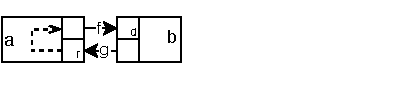
\includegraphics[width=0.5\textwidth]{images/simple_example.pdf}
  \caption{A co-simulation scenario with two SUs $a$ and $b$. 
  The dashed arrows denote feed-through connections, the ports are represented as small squares, the instrumentation of an input port is denoted by the letters $r$ (reactive) or $d$ (delayed).
  The solid arrows $f$ and $g$ represent couplings.}
  \label{fig:simpleexample}  
\end{figure}

%The instrumentation describes the input approximation functions of the different SUs.

\subsection{Co-simulation Algorithms}\label{sc:cosimalgo}
An \emph{orchestrator} simulates a scenario by executing a \emph{co-simulation algorithm}.
A co-simulation algorithm consists of an initialization procedure and a co-simulation step~\cite{FMI2014}.
This work focuses on the co-simulation step, which we refer to as ``the algorithm'' in the paper.

The state of a co-simulation scenario is defined as the combination of the states of its subcomponents:

\begin{definition}[Abstract SU State]\label{def:runtime_state}
  The observable abstract state $\runstate{}$ of an SU $\mathcal{SU}_c$ in a scenario $\mathcal{S}$ is an element of the set $\runstateset{c} = \timebase \times \runstateset{\inputs{c}} \times \runstateset{\outputs{c}} \times \runstateset{V_c}$, where:
  \begin{compactitem}
    \item $\runstateset{\inputs{c}} : \inputs{c} \to \timebase$ is a function mapping each input port to a timestamp.  
    \item $\runstateset{\outputs{c}} : \outputs{c} \to \timebase$ is a function mapping each output port to a timestamp.  
    \item $\runstateset{V_c} : \variables{c} \to \values$ is a function mapping each port to a value.  
  \end{compactitem}
  The first component of the abstract state denotes the time of the SU.
\end{definition}

We use the abstract state $\runstate{c}$ of an SU $c$ instead of the internal state $\state{c}$ since the orchestrator cannot observe the latter.

\begin{definition}[Abstract Co-simulation State]\label{def:cosimstate}
  The abstract co-simulation state $\runstate{\scenario}$ of a scenario $\scenario =\tuple{\fmus, \{\mathcal{SU}_c\}_{c \in \fmus}, \coupling, \mayReject, \allreactivity, \allfeedthroughs}$ is an element of the set $\runstateset{\scenario} = \ftime \times \runstateset{\allinputs} \times \runstateset{\alloutputs} \times \runstateset{V}$
  where:
  \begin{itemize}
    \item $\ftime : \fmus \to \timebase$ is a function, where $\ftime(c)$ denotes the current simulation time of $\mathcal{SU}_c$.
    We denote by a time value $t \in \timebase$ the function $\lambda c.t$, which we use if all SUs are at the same time.
    \item $\runstateset{\allinputs} = \prod_{c \in \fmus} \runstateset{\inputs{c}}$ maps all inputs of the scenario to a timestamp. 
    \item $\runstateset{\alloutputs} = \prod_{c \in \fmus} \runstateset{\outputs{c}}$ maps all outputs of the scenario to a timestamp. 
    \item $\runstateset{V} =  \prod_{c \in \fmus} \runstateset{V_c}$ maps all ports of the scenario to a value. 
  \end{itemize}
\end{definition}

A co-simulation step $P$ is a sequence of operations that takes a co-simulation from one consistent state to another consistent state.
We write $ s \xrightarrow[\text{}]{\text{P}} s'$ if executing the co-simulation step $P$ from the state $s$ results in the state $s'$.

\begin{definition}[Co-simulation Step]\label{def:comsim_step}
  A \emph{co-simulation step} $P$ is a sequence of SU actions that takes a consistent co-simulation state to another consistent  co-simulation state. 
  The state of the co-simulation is consistent if all input ports have a source, and all coupled ports have the same value.
  Formally:
  \begin{align*}
    &\qquad \qquad \qquad \qquad \tuple{t,\runstate{\allinputs}, \runstate{\alloutputs},\runstate{V}}
    \xrightarrow[\text{}]{\text{P}} \tuple{\after{t},\after{\runstate{\allinputs}}, \after{\runstate{\alloutputs}},\after{\runstate{V}}} \\
    &\implies
    (\fpreCoSimStep(\tuple{t,\runstate{\allinputs}, \runstate{\alloutputs},\runstate{V}}) 
    \implies
    (\fpreCoSimStep(\tuple{\after{t},\after{\runstate{\allinputs}}, \after{\runstate{\alloutputs}},\after{\runstate{V}}})
    \land \after{t} > t))
  \end{align*}
  where consistent is defined as:
  \begin{align*}
    &\fpreCoSimStep(\tuple{t,\runstate{\allinputs}, \runstate{\alloutputs},\runstate{V}}) \triangleq 
    (\forall \inputvar{c} \in \allinputs
    \exists \outputvar{d} \in \alloutputs 
    \cdot \coupling(\inputvar{c}) = \outputvar{d})  \nonumber \\
    &\qquad \qquad \qquad \qquad \qquad \land
    (\forall \inputvar{c}, \outputvar{d} \cdot \coupling(\inputvar{c}) = \outputvar{d} 
    \implies
    \runstate{V}(\inputvar{c}) = \runstate{V}(\outputvar{d}))
  \end{align*}
\end{definition}


Informally, the co-simulation step advances the scenario from an initial state at time $t$ to a final state at time $t+H, \textrm{ where } H > 0$, and ensures that the coupling restrictions are satisfied at both the initial and the final state.

\Cref{fig:algorithms} shows three different co-simulation steps of the scenario in \cref{fig:simpleexample} that are allowed by the FMI standard 2.0~\cite{FMI2014}. 

\begin{figure}[htb]
  \centering
  \begin{minipage}[t]{.325\textwidth}
    \begin{algorithm}[H]
      \caption{}
      \label{alg:algorithm_1}
      \begin{algorithmic}[1]
        \scriptsize
        \State $(\stateafter{A}{H},H) \gets \fdoStep{A}(\stateafter{A}{0}, H)$
        \State $(\stateafter{B}{H},H) \gets \fdoStep{B}(\stateafter{B}{0}, H)$
        \State $f_{v} \gets \fget{A}(\stateafter{A}{H}, \outputvar{f})$
        \State $g_{v} \gets \fget{B}(\stateafter{B}{H}, \outputvar{g})$
        \State $\stateafter{B}{H} \gets \fset{B}(\stateafter{B}{s}, \inputvar{f}, f_{v})$
        \State $\stateafter{A}{H} \gets \fset{A}(\stateafter{A}{H},\inputvar{g},g_{v})$
      \end{algorithmic}
    \end{algorithm}
  \end{minipage}
  \begin{minipage}[t]{0.325\textwidth}
    \begin{algorithm}[H]
      \caption{}
      \label{alg:algorithm_2}
      \begin{algorithmic}[1]
        \scriptsize
        \State $(\stateafter{B}{H},H) \gets \fdoStep{B}(\stateafter{B}{0}, H)$
        \State $(\stateafter{A}{H},H) \gets \fdoStep{A}(\stateafter{A}{0}, H)$
        \State $g_v \gets \fget{B}(\stateafter{B}{H}, \outputvar{g})$
        \State $\stateafter{A}{H} \gets \fset{A}(\stateafter{A}{H}, \inputvar{g}, g_v)$
        \State $f_v \gets \fget{A}(\stateafter{A}{H}, \outputvar{f})$
        \State $\stateafter{B}{H} \gets \fset{B}(\stateafter{B}{H}, \inputvar{f}, f_v)$
      \end{algorithmic}
    \end{algorithm}
  \end{minipage}
  \begin{minipage}[t]{0.325\textwidth}
    \begin{algorithm}[H]
      \caption{}
      \label{alg:algorithm_3}
      \begin{algorithmic}[1]
        \scriptsize
        \State $(\stateafter{B}{H},H) \gets \fdoStep{B}(\stateafter{B}{0}, H)$
        \State $g_v \gets \fget{B}(\stateafter{B}{H}, \outputvar{g})$
        \State $\stateafter{A}{0} \gets \fset{A}(\stateafter{A}{0}, \inputvar{g}, g_v)$
        \State $f_v \gets \fget{A}(\stateafter{A}{0}, \outputvar{f})$
        \State $\stateafter{B}{H} \gets \fset{B}(\stateafter{B}{H}, \inputvar{f}, f_v)$
        \State $(\stateafter{A}{H},H) \gets \fdoStep{A}(\stateafter{A}{0}, H)$
      \end{algorithmic}
    \end{algorithm}
    \vspace{4pt}
  \end{minipage}
  \vspace{-2em}
  \caption{Three co-simulation algorithms of the scenario in \cref{fig:simpleexample} conforming to the FMI Standard (version 2.0).}
  \label{fig:algorithms}
\end{figure}

Although the three algorithms satisfy \cref{def:comsim_step} and consist of the same actions, they are not equivalent, and simulating with one algorithm instead of one of the others could change the co-simulation result as shown in \cite{Gomes2019c,hansen_verification_2021}. 
To differentiate between them, we need to consider the semantics of the different actions described in \cref{def:fmu}, which we describe in \cref{def:getout,def:setin,def:step}.

We base our semantics on \cite{Gomes2019a,hansen_verification_2021} to which we refer for more information.

\begin{definition}[Get Action]\label{def:getout}   
  To obtain a value from an output port $\outputvar{}$ of an SU at time $t$ using the action $\fget{}(\stateafter{}{t},\outputvar{})$ changes the state of the SU according to:
  \begin{align*}
    \runstate{} 
    \xrightarrow[\text{}]{\fget{}(\stateafter{}{t}, \outputvar{})} 
    (v,\after{\runstate{}})
    \implies 
    \fpreget{}(\outputvar{}, \runstate{})
    \land
    \fpostget{}(\outputvar{}, \runstate{}, \after{\runstate{}}, v)
  \end{align*}
  Where:
  \begin{align*}
    &\fpreget{}(\outputvar{}, \tuple{t,\runstate{\inputs{}}, \runstate{\outputs{}}, \runstate{V}}) \triangleq
    \runstate{\outputs{}}(\outputvar{}) < t \land
    \forall \inputvar{} \in \allfeedthroughs(\outputvar{}) \cdot \runstate{\inputs{}}(\inputvar{}) = t 
  \end{align*}
  The precondition (above) states that no value must have been obtained from the output $\outputvar{}$ since the SU was stepped, formally described as $\runstate{\outputs{}}(\outputvar{}) < t$.
  Furthermore, it requires that all the inputs that feed through to $\outputvar{}$ have been updated, so they are at time $t$.
  The postcondition (below) ensures that the output is advanced time $t$.
  \begin{align*}
    &\fpostget{}(\outputvar{}, \tuple{t,\runstate{\inputs{}}, \runstate{\outputs{}}, \runstate{V}}, 
    \tuple{t,\runstate{\inputs{}}, \after{\runstate{\outputs{}}}, \runstate{V}}, v) \triangleq 
    \after{\runstate{\outputs{}}}(\outputvar{}) = t \nonumber \\
    & \qquad \qquad \qquad \qquad \qquad 
    \land 
    \forall \outputvar{m} \in (\outputs{} \setminus \outputvar{}) \cdot 
    \after{\runstate{\outputs{}}}(\outputvar{m}) =
    \runstate{\outputs{}}(\outputvar{m})
  \end{align*}
\end{definition}

\begin{definition}[Set Action]\label{def:setin}
  Setting a value $\tuple{t_{v}, x}$ on the input port $\inputvar{}$ of an SU using $\fset{}(\stateafter{}{t}, \inputvar{}, \tuple{t_{v}, x})$ updates the time and value of the input port $\inputvar{}$ such that it matches $\tuple{t_{v}, x}$, formally:
  \begin{align*}
    \runstate{} 
    \xrightarrow[\text{}]{\fset{}(\stateafter{}{t}, \inputvar{}, \tuple{t_{v}, x})} 
    \after{\runstate{}}
    \implies 
    \fpreset{}(\inputvar{}, \runstate{})
    \land
    \fpostset{}(\inputvar{}, \inputV, \runstate{}, \after{\runstate{}})
  \end{align*}
  Where:
    \begin{align*}
      &\fpreset{}(\inputvar{}, \tuple{t_{v},x}, \tuple{t,\runstate{\inputs{}}, \runstate{\outputs{}}, \runstate{V}}) \triangleq 
      \runstate{\inputs{}}(\inputvar{}) < t_{v} \nonumber \\
      & \qquad \qquad \qquad \qquad \qquad
      \land 
      ((\allreactivity(\inputvar{c}) \land \runstate{\inputs{}}(\inputvar{}) = t) 
      \lor (\neg\allreactivity(\inputvar{c}) \land \runstate{\inputs{}}(\inputvar{}) < t))
    \end{align*}
    The precondition says that the input must not have been assigned a new value since the SU was stepped, formally $\runstate{\inputs{}}(\inputvar{}) < t_{v}$.
    Furthermore, it requires that the value $\tuple{t_{v},x}$ respects the instrumentation of the input.
    The postcondition (below) ensures the value and time of the input $\inputvar{}$ is updated so it matches the value assigned on the input. 
    \begin{align*}
      &\fpostset{}(\inputvar{}, \tuple{t_{v},x}, \tuple{t,\runstate{\inputs{}}, \runstate{\outputs{}}, \runstate{V}}, 
      \tuple{t, \after{\runstate{\inputs{}}} \runstate{\outputs{}}, \after{\runstate{V}}}) \triangleq 
      t_{v} = \after{\runstate{\inputs{}}}(\inputvar{})
      \nonumber\\
      &\qquad \qquad \qquad \land
      (\forall \inputvar{m} \in (\inputs{} \setminus \inputvar{}) \cdot 
      \after{\runstate{\inputs{}}}(\inputvar{}) =
      \runstate{\inputs{}}(\inputvar{})) \land
      \after{\runstate{V}}(\inputvar{}) = x 
    \end{align*}
  \end{definition}

  \begin{definition}[Step Computation]\label{def:step}
    To step an SU using $\fdoStep{}(\stateafter{}{t}, H)$ advances the state of the SU by $H$, formally:
    \begin{align*}
      \runstate{} 
      \xrightarrow[\text{}]{\fdoStep{}(\stateafter{}{t}, H)} 
      \after{\runstate{}}
      \implies 
      \fpredoStep{}(H, \runstate{})
      \land
      \fpostdoStep{}(H, \runstate{}, \after{\runstate{}})
    \end{align*}
    Where:
    \begin{align*}
      &\fpredoStep{}(H, \tuple{t,\runstate{\inputs{}}, \runstate{\outputs{}, \runstate{V}}}) \triangleq 
      \forall \inputvar{} \in \inputs{}
      \cdot 
      ((\allreactivity(\inputvar{}) \land t_{SU} + H = \runstate{\inputs{}}(\inputvar{}))
      \nonumber \\
      &\qquad \qquad \qquad \qquad \qquad \qquad \qquad \qquad \qquad 
      \lor 
      (\neg \allreactivity(\inputvar{}) \land t_{SU} = \runstate{\inputs{}}(\inputvar{})))
    \end{align*}
    The precondition (above) states that all the SU's inputs have been updated according to their instrumentation.  
    The postcondition (below) ensures that the time of the SU advances by $H$.
    \begin{align*}
      &\fpostdoStep{}(H, \tuple{t,\runstate{\inputs{}}, \runstate{\outputs{}}, \runstate{V}}, \tuple{t',\runstate{\inputs{c}}, \runstate{\outputs{}}, \after{\runstate{V_c}}}) \triangleq t + h' = t' \land h' \leq H
    \end{align*}
  \end{definition}

An algorithm $P$ must satisfy \cref{def:comsim_step} while respecting the defined semantics.
This means that \cref{alg:algorithm_3} is correct, while \cref{alg:algorithm_2,alg:algorithm_1} are incorrect since they do not respect the semantics.
%For example, \cref{alg:algorithm_2} tries to perform a $\fdoStep{A}$ action in line 2 without respecting the reactive input $\inputvar{g}$ since the state of SU $A$ $\runstate{A} = \tuple{0,\{\inputvar{g} \to 0 \}, \{\outputvar{f} \to 0 \}, \dontcare}$ does not contain $\{\inputvar{g} \to H \}$.
%Intuitively, we try to step SU $A$ without having provided it with a value on the reactive input $\inputvar{g}$; this is an apparent violation of $\fpredoStep{A}$.
% \subsection{Complex Co-simulation Scenarios}
% Complex co-simulation scenarios are subject to algebraic loops or step rejections~\cite{thrane2021,Kubler2000,Oakes2021}.
% An algebraic loop denotes a cyclic dependency between the SUs; real-world examples include the suspension system of a car~\cite{thranefmi-based2020}.
% % Algebraic loops can be detected as a non-trivial strongly connected component of the graph constructed using the rules \cite[Definition 15]{Gomes2019c}.
% Step rejections, triggered by error estimation inside the SU, need special attention because they can result in a co-simulation step where the SUs do not move in lockstep.
% A complex scenario is simulated using an iterative co-simulation algorithm that adapts to the behavior of the SUs to satisfy the constraints associated with each SU, account for possible step rejections, and solve algebraic loops. 
%The orchestrator achieves this by finding a correct valuation of all inputs and outputs in the scenario~\cite{thrane2021}.
%The valuation defines the step duration and the current attempt to solve the scenario's algebraic loops. 
%A correct valuation ensures that all SUs agree on the step duration and solves all algebraic loops by finding a fixed point.
%A complex co-simulation scenario can only be correctly simulated using a correct valuation.
%The orchestrator must find a correct valuation in every co-simulation step because it depends on the current internal state of the SUs, which varies from one co-simulation step to the next.
%The process for finding a correct valuation is due to space limitations not covered here; we refer interested readers to \cite{thrane2021,Kubler2000}.
% \subsection{Design Space Exploration}
% Design space exploration is a technique for evaluating how different combinations of parameters (designs) affect the system's performance to determine which parameter combinations are ``optimal''~\cite{kang_approach_2011}.
% The parameters of an SU are constants that configure the SU's behavior; an example is the parameter \texttt{flow} described in \cref{ex:simulationunits}.
% Design space exploration can roughly be divided into two phases a search and a design evaluation.
% The search finds the different combinations of parameters (designs) while the design evaluation evaluates them.
% Design space exploration can be used in the context of co-simulation and digital twins, where it provides a cheap way to explore the consequence of different design decisions~\cite{gamble_design_2014,dse}.

\subsection{Problem Statement}
The two key problems in co-simulation that we addresses in this paper (in addition to the formalization of a co-simulation) are:
\begin{compactenum}
  \item Given a scenario $\scenario$ synthesize an implementation-aware co-simulation algorithm $P$ for $\scenario$.
  That is, find the sequence of SU actions $P$ so that running $P$ on $\scenario$ satisfies \cref{def:comsim_step} while respecting the semantics.
  This includes solving possible algebraic loops and performing step negotiation to ensure that all SUs move in lockstep.
  \item Given a \emph{parametric} or \emph{partially instrumented} scenario $\scenario$, where some SU parameters are unknown and where the instrumentation is incomplete, i.e., not all input ports have been declared ether \emph{reactive} or \emph{delayed}, find concrete values for the parameters, and concrete instrumentation of the input ports, such that the resulting \emph{instrumented} scenario represents a system with desirable properties.
\end{compactenum}
